\subsection{Orientering af SIFT punkter}
Orienteringen af punkter skal bruges i deskriptoren, for at den kan være invariant overfor rotation. Skridtet her, kan beskrives ved:
\begin{equation}
Orientering(p, \sigma) = \theta
\end{equation}
Hvor $p$ er interessepunktet, $\sigma$ er skalaen, og $\theta$ er orienteringen af punktet $p$. 
\\
\\
Et 16x16 dataindsamlingsvindue er placeret omkring interessepunktet, på den skala og tilsvarende billede, interessepunktet er fundet på. For alle punkte i dataindsamlingsvinduet, er en størrelsen på en gradient, og dens orientering beregnet:
\begin{equation}
m(x,y) = \sqrt{(L(x + 1, y) - L(x - 1, y)^2 + (L(x, y + 1) - L(x, y - 1))^2  } 
\label{magnitudepoint}
\end{equation}
\begin{equation}
o(x,y) = tan^{-1}((L(x + 1, y) - L(x - 1, y))^2 + (L(x, y + 1) - L(x, y - 1))^2 ) 
\label{orientationpoint}
\end{equation}
$m$ er størrelsen af en gradient, og $o$ er gradientens retning. alle punkter indenfor dataindsamlingsvinduet, skal gives som input til \eqref{magnitudepoint} og \eqref{orientationpoint}, for at skabe et gradientvindue $g$ og orienteringsvindue $v$. Begge vinduer har størrelse 16x16. $g$ skal herefter foldes med et Gaussfilter hvor $\sigma_{Gauss} = 1.5\sigma_{point} $, med størrelse 16x16.
\\
\\
Der skal oprettes et orienteringshistogram $H$, med 36 indgange. Alle gradienter med orientering $v$, skal tilføjes vægtet af $g$ til $H$. En indgang i $H$, dækker en vinkel på $10^{\circ}$. F.eks. skal alle gradienter med vinkler mellem  $0^{\circ}-10^{\circ}$, tilføjes vægtet, til $H_1$, osv.. Dette resulterer i et orienteringshistogram, og den indgang i histogrammet med størst værdi, bliver bearbejdet. Lowe foreslår, at alle indgange i histogrammet, der ligger indenfor 80\% af det højeste punkt, bliver nye features - dette er undladt her, for at undgå at få for mange matches.
\\
Der skal nu foretages en interpolation, omkring den indgang i histogrammet, med størst værdi, for at få et mere præcist estimat af $\theta$.

\begin{figure}[H]
    \centering
    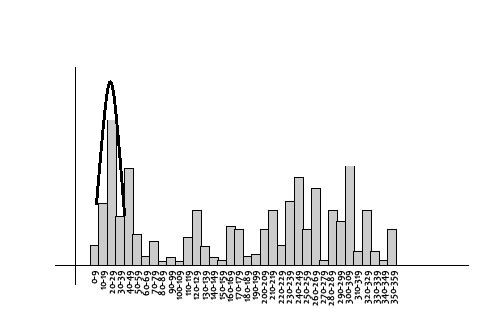
\includegraphics[width=0.45\textwidth]{fig/sift-orientation-histogram.jpg}
     \vspace{-1em}
    \begin{center}    
       \caption{\textcolor{gray}{\footnotesize \textit{Histogrammet $H$ afbilledet, sammen med en andengradsligning. Andengradsligningen er beregnet over den største indgang i $H$}}}
    \label{histogramheight}
     \end{center}
     \vspace{-2.5em}
  \end{figure} \noindent

Dette ses på figur \ref{histogramheight}: En andengradsligning er blevet tilnærmet den største værdi af $H$. Estimering af andengradspolynomiet sker over den største værdi i $H$, og dennes umiddelbare venstre og højre nabo.

\subsection*{Algoritme}
\begin{enumerate}
\item Dataindsamlingsvindue placeres omkring interessepunkt, på samme skala og variant af billedet, som $\sigma$ foreskriver.
\item \eqref{magnitudepoint}, \eqref{orientationpoint} bruge til at udregne alle størrelser og orienteringer af gradienter, $g$, $v$, respektivt. $g$ foldes, så: $g = G(x,y,1.5\sigma)$.
\item Værdiene i $g$ adderes på indgange i histogrammet $H$, afhængigt af deres tilsvarede orientering i $v$.
\item En interpolation laves omkring den største værdi i $H$ og dens tætteste naboer. Denne værdi returneres
\end{enumerate}
